\section{A finite paired pulse generates a standing residual}\label{sec:pulse}
The preceding free waves were independently prepared. We next derive what the retained source interface generates from rest under the SRG-07 calibration.~\cite{SRG07} Fix $\epsilon=L/32$, $T=L/c$, $\omega=c/R=2\pi/T$, and
\begin{equation}\label{eq:pulse}
 h(t)=\begin{cases}\sin^2(\pi t/T),&0\le t\le T,\\0,&\text{otherwise},\end{cases}
 \qquad f_\pm(t)=(F_s\pm F_a)h(t),\qquad p=r=0\quad(t\le0).
\end{equation}
Here $F_s,F_a$ are real constants. The zero extension is $C^1$, since both $h$ and $h'$ vanish at the endpoints. Its exactly one-circuit duration is a temporal calibration, not a native drive period. Define $C_g=\sqrt{3/7}$, $S_g=2/\sqrt7$ and $B_n=\sinc^2(n\pi/32)$, with $b=B_1=0.996791364044961\ldots$.

The controls S, A, M+, M- and ZERO use
\begin{equation}\label{eq:pulsecontrols}
 (F_s,F_a)/F_0=(1,0),(0,1),(1,1)/\sqrt2,(1,-1)/\sqrt2,(0,0)
\end{equation}
with one common $F_0>0$. M+ is upper-only, M- lower-only. They are names for pulse combinations, not additional native macro families. Expanding $f_+^2+f_-^2$ and integrating $\sin^4$ gives
\begin{equation}\label{eq:drivenorm}
 \int_0^T(f_+^2+f_-^2)\dd t=\frac{3T}{4}(F_s^2+F_a^2).
\end{equation}
All four nonzero controls have equal squared drive norm, which does not imply equal signed work.

\subsection{All modes during forcing; exact cancellation at switch-off}
Let $G=(F_s+F_a)b_++(F_s-F_a)b_-$. Its Fourier coefficients are
\begin{equation}\label{eq:G}
 G_n=\frac{2(-1)^n}{L}B_n[F_s\cos(n\theta)+\ii F_a\sin(n\theta)].
\end{equation}
For $0\le v\le T$, introduce the entire limiting primitive
\begin{equation}\label{eq:J}
 E_m(v)=\begin{cases}(e^{\ii m\omega v}-1)/(\ii m\omega),&m\ne0,\\v,&m=0,\end{cases}
 \qquad J_n(v)=\tfrac12E_n(v)-\tfrac14E_{n+1}(v)-\tfrac14E_{n-1}(v).
\end{equation}
For $t\ge0$ set $v=\min(t,T)$ and $Z_n=e^{-\ii n\omega t}J_n(v)$. Direct use of the two characteristics gives
\begin{equation}\label{eq:transient}
 p_n(t)=G_n\Re Z_n,\qquad r_n(t)=\ii G_n\Im Z_n,
 \qquad p_0(t)=\frac{F_s}{L}\left(v-\frac{\sin\omega v}{\omega}\right),\quad r_0=0.
\end{equation}
The spatial form, with periodic arguments, is
\begin{equation}\label{eq:directpulse}
 \binom p r(s,t)=\frac12\sum_{\sigma=\pm1}\binom1\sigma
 \int_0^{\min(t,T)}G(s-\sigma c(t-u))h(u)\dd u.
\end{equation}
These formulas retain the full spatial spectrum. The finite tent is not a hard cutoff, and generally $J_n(v)\ne0$ for higher modes before switch-off.

\begin{theorem}[One-circuit pulse selection]\label{thm:pulsemoments}
For every integer $n$ and $\sigma=\pm1$,
\begin{equation}\label{eq:pulsemoments}
 \int_0^T h(u)e^{\sigma\ii n\omega u}\dd u
 =\frac T2\delta_{n0}-\frac T4(\delta_{n1}+\delta_{n,-1}).
\end{equation}
Consequently at $t=T$,
\begin{equation}\label{eq:switchoff}
 p_0=F_s/c,\quad r_n=0\ (n\in\mathbb Z),\quad
 p_1=\frac b{2c}(F_sC_g+\ii F_aS_g),\quad p_{-1}=\overline{p_1},\quad p_n=0\ (|n|\ge2).
\end{equation}
\end{theorem}
\begin{proof}
Write $h(u)=1/2-e^{\ii\omega u}/4-e^{-\ii\omega u}/4$ on its support. Every nonconstant integer exponential integrates to zero on $[0,T]$; the constant integrates to $T$. Applying this to each of the three terms gives \eqref{eq:pulsemoments} for every integer, including $0,\pm1$. There is no singular denominator: its value is precisely the $E_0$ branch of \eqref{eq:J}. At $T$, all free phase factors $e^{\pm\ii n\omega T}$ equal one, and the two signed moments agree. Thus their half-difference, the $r_n$ coefficient, is zero. Their half-sum gives $p_n=G_nJ_n(T)$. Substituting \eqref{eq:G} at $n=0,1$ gives \eqref{eq:switchoff} and real conjugacy gives $n=-1$.
\end{proof}

\begin{corollary}[Uniquely generated continuation]\label{cor:standing}
For $\tau=t-T\ge0$, the resulting free continuation is
\begin{equation}\label{eq:residual}
 \begin{aligned}
 p&=\frac{F_s}{c}+\frac bc(F_sC_g\cos\chi-F_aS_g\sin\chi)\cos\omega\tau,\\
 r&=\frac bc(F_sC_g\sin\chi+F_aS_g\cos\chi)\sin\omega\tau.
 \end{aligned}
\end{equation}
At the shared $T$ reference its first-harmonic amplitudes are
\begin{equation}\label{eq:pulseamplitudes}
 a_+=\frac b{2c}(F_sC_g-\ii F_aS_g),\qquad
 a_-=\frac b{2c}(F_sC_g+\ii F_aS_g).
\end{equation}
\end{corollary}
\begin{proof}
The mean is constant after forcing. Evolving each surviving Fourier coefficient with unforced C1 gives $p_1(T+\tau)=p_1(T)\cos\omega\tau$ and $r_1(T+\tau)=-\ii p_1(T)\sin\omega\tau$. Combining conjugate spatial modes gives \eqref{eq:residual}; comparison with \eqref{eq:freefamily} gives \eqref{eq:pulseamplitudes}. It matches the complete switch-off state and solves C1, so uniqueness identifies it as the continuation.
\end{proof}

Here $a_-=p_1(T)$, not $a_+$. For real $F_s,F_a$, the amplitudes are conjugates and their magnitudes agree. S produces a mean plus cosine standing pattern; A produces a mean-free sine standing pattern. M$\pm$ yield standing $p$ harmonics proportional to $\cos(\chi\pm\theta)$. The shift records contact geometry, not opposite circulation. Higher-mode cancellation is a property of the completed pulse and its exact duration; it is neither damping nor a universal selection law.

\begin{theorem}[Common-envelope obstruction at every time]\label{thm:commonzero}
For zero preparation and any real separable forcing $G(s)h(t)$ with the finite-profile regularity above, $\Jflux(t)=0$ at every time, including during forcing. This includes all controls in \eqref{eq:pulsecontrols}.
\end{theorem}
\begin{proof}
The modal Duhamel solution has $p_n=G_n A_n$ and $r_n=-\ii G_n B_n^{\rm time}$, where $A_n=\int_0^t h(u)\cos[ck_n(t-u)]\dd u$ and $B_n^{\rm time}=\int_0^t h(u)\sin[ck_n(t-u)]\dd u$ are real. Hence $\Re(p_n\overline{r_n})=0$ for every mode. The mean $r_0$ is zero. Parseval, justified by $L^2$ convergence and Cauchy--Schwarz for the coefficient product, gives $c\int pr\dd s=0$. This proves an all-time statement, stronger than equality of the two residual magnitudes. Local flux need not vanish.
\end{proof}

\subsection{Signed work, storage and port interference}
\begin{proposition}[Pulse work and storage]\label{prop:pulsework}
For \eqref{eq:pulse}, the final storage and integrated signed source work are
\begin{equation}\label{eq:pulsestorage}
 E_f=W_{\rm src}=\frac L{c^2}\left[\frac12F_s^2+
 \frac{b^2}{4}(C_g^2F_s^2+S_g^2F_a^2)\right].
\end{equation}
The antisymmetric control A has negative instantaneous source work on an interval immediately before $T$, although its total work is positive.
\end{proposition}
\begin{proof}
Integrating the square of \eqref{eq:residual} uses $\int\sin\chi=\int\cos\chi=\int\sin\chi\cos\chi=0$ and $\int\sin^2\chi=\int\cos^2\chi=L/2$. The mean/harmonic and symmetric/antisymmetric cross terms vanish by these identities, giving the displayed $E_f$.

Independently integrate the actual source work. Put $I_n=J_n(T)$ and define
\[
 A_n(t)=\int_0^t h(u)\cos[n\omega(t-u)]\dd u.
\]
The source power is $Lh(t)\sum_n|G_n|^2A_n(t)$. Symmetry of the cosine kernel gives
\[
 \int_0^T h(t)A_n(t)\dd t
 =\frac12\int_0^T\int_0^T h(t)h(u)\cos[n\omega(t-u)]\dd u\dd t
 =\frac12|I_n|^2.
\]
Thus $W_{\rm src}=(L/2)\sum_n|G_n|^2|I_n|^2$. The finite-profile coefficient decay and bounded temporal integrals justify interchanging sum and integrals. Inserting \eqref{eq:pulsemoments} produces exactly \eqref{eq:pulsestorage}, without defining work by endpoint storage.

Before multiplication by the endpoint envelope, the limiting source trace is
\begin{equation}\label{eq:negativework}
 \int Gp(T)\dd s=\frac2c\left[F_s^2-b^2(C_g^2F_s^2+S_g^2F_a^2)\right].
\end{equation}
This follows by pairing the mean and first harmonics of $G$ and $p(T)$. For A it is $-2b^2S_g^2F_0^2/c<0$. The trace is continuous in time, and $h(t)>0$ just before $T$. Hence $h(t)\int Gp(t)\dd s<0$ on a final open interval. The endpoint itself has zero power because $h(T)=0$.
\end{proof}

For S and the positive single-port controls, $G\ge0$, and \eqref{eq:directpulse} implies $p\ge0$. Their instantaneous work is nonnegative. These different signs arise from the prescribed sources, with no negative storage. The comparison in Table~\ref{tab:pulsestorage} uses a single unit $F_0^2L/c^2$.
\begin{table}[htbp]\centering
\begin{tabular}{lrrr}\toprule
Control & Mean storage & Harmonic storage & Total storage / signed work\\\midrule
S & .5000000000 & .1064563954 & .6064563954\\
A & 0 & .1419418605 & .1419418605\\
M+ & .2500000000 & .1241991279 & .3741991279\\
M- & .2500000000 & .1241991279 & .3741991279\\
ZERO & 0 & 0 & 0\\\bottomrule
\end{tabular}
\caption{Same squared drive norm for nonzero controls; unequal delivered work. The A/S harmonic-storage ratio is exactly $4/3$, but S has larger total storage because its mean remains.}\label{tab:pulsestorage}
\end{table}

Let $\alpha_S=1/2+3b^2/28$ and $\alpha_A=b^2/7$. In terms of actual port amplitudes $F_\pm=F_s\pm F_a$, the account becomes
\begin{equation}\label{eq:portcross}
 E_f=\frac L{4c^2}\left[(\alpha_S+\alpha_A)(F_+^2+F_-^2)
 +2(\alpha_S-\alpha_A)F_+F_-\right].
\end{equation}
Thus diagonalization in reflection sectors does not make physical port work independent. The mixed term is nonzero and cannot be replaced by absolute values.

\begin{figure}[htbp]\centering
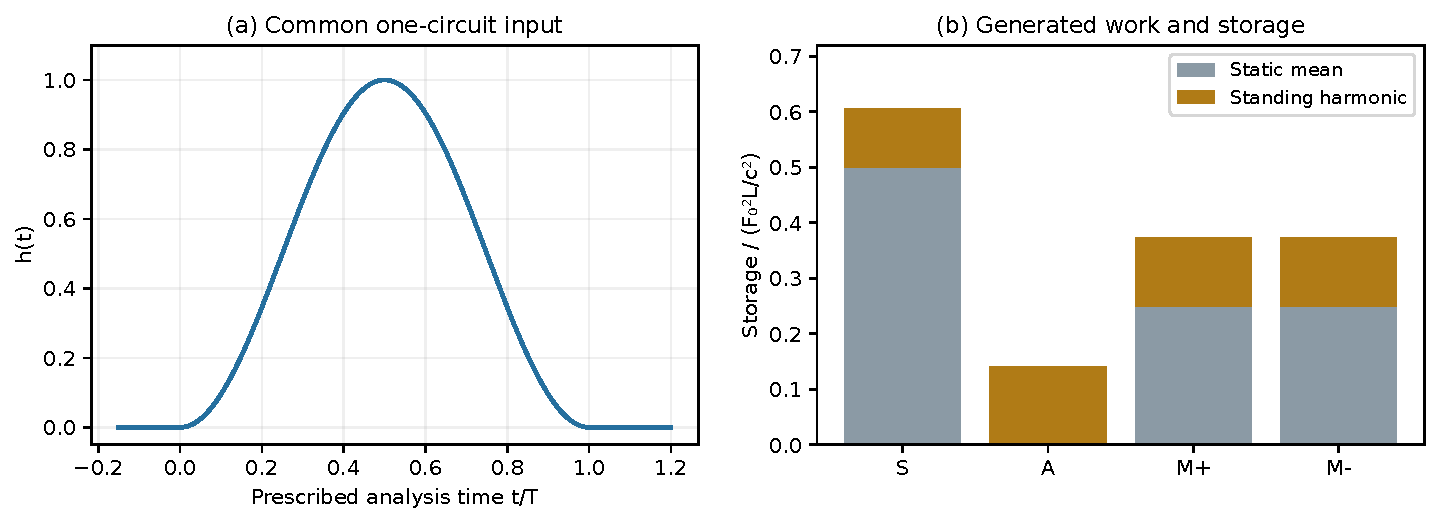
\includegraphics[width=\textwidth]{figures/pulse.pdf}
\caption{Common-pulse calibration and its generated storage, from retained SRG-07 data. The waveform is a prescribed input, not a simulated native trajectory. Bars retain the static mean and share the unit $F_0^2L/c^2$. All four nonzero cases have zero integrated directional bias at all times.}\label{fig:pulse}
\end{figure}

\subsection{Complete late records and the two-real-coefficient inverse}
Across the full fixed array,
\begin{equation}\label{eq:latewindow}
 D_{\max}=4+K+R=5.29316210017650\ldots,\qquad
 I_{\rm late}=[T+D_{\max}/c_e,T+D_{\max}/c_e+T].
\end{equation}
The maximum is attained at R3:06. Since $d_X(s)\le D_{\max}$, every retarded argument in this common window is at least $T$. At zero exterior delay the additional offset is zero. The phase reference remains $t-T$ at every site; it is not aligned independently to local delay.

Use the accepted unit-$g_o$ matrices $Q_X(\nu)$ and the accepted zero-delay moments to define
\begin{equation}\label{eq:sourceN}
 N=\frac b2\begin{pmatrix}C_g&-\ii S_g\\C_g&\ii S_g\end{pmatrix},\quad
 D_X=S_m(X,0)+C_m(X,0)=\frac1{4\pi}\int_\Gamma d_X^{-1}\dd s>0.
\end{equation}
For $\mathbf f=(F_s,F_a)\tr/F_0$, the complete late record is
\begin{equation}\label{eq:laterecord}
 \frac{Y_X(t)}{g_oF_0/c}
 =\begin{pmatrix}D_X&0\\0&0\\0&0\\0&0\end{pmatrix}\mathbf f
 +\Re\{Q_X(\nu)N\mathbf f\,e^{\ii\omega(t-T)}\}.
\end{equation}
There is no static vector term because $\bar r=0$. Earlier records require \eqref{eq:composition} with the actual pulse, including its transient higher modes; the late expression is not a prehistory substitute.

\begin{theorem}[Causal null and calibrated pulse identification]\label{thm:pulseinverse}
Under the common-pulse controls, equatorial scalar reception satisfies $U_A=0$ and $U_{M+}=U_{M-}=U_S/\sqrt2$ throughout the causal history, for every $c_e$. At $\nu=0,1$, a full harmonic record at any retained site identifies both real coefficients $F_s,F_a$. A single off-height scalar harmonic has only real rank one, while its calibrated DC-plus-harmonic record has real rank two. The fixed off-height mirror pair or each off-height H ring has harmonic scalar rank two. Coplanar scalar stacks have rank one even with DC.
\end{theorem}
\begin{proof}
Proposition~\ref{prop:parity} makes $p_A$ odd under $s\mapsto L-s$. At an equatorial site the distance and delay are even under that reflection, so opposite source points are read at the same time and cancel. Linearity gives the M$\pm$ identity for the entire history.

Substitute \eqref{eq:pulseamplitudes} into \eqref{eq:reduction}. In the common scale the scalar harmonic is
\begin{equation}\label{eq:pulsescalar}
 \widehat U/(g_oF_0/c)=bH(C_g f_s^{\rm norm}\cos\phi-S_g f_a^{\rm norm}\sin\phi),
\end{equation}
where $f_s^{\rm norm}=F_s/F_0$, $f_a^{\rm norm}=F_a/F_0$. This is one real combination times a known complex scalar, so it has real rank one. At off-height sites $\sin\phi\ne0$; DC determines $F_s$ since $D_X>0$, after which \eqref{eq:pulsescalar} determines $F_a$. The two mirror harmonic rows are proportional to $(C_g\cos\phi,\mp S_g\sin\phi)$, both factors nonzero at the declared pair. The same nonparallel-angle argument as in Theorem~\ref{thm:height} treats each off-height ring. At equator the $F_a$ column vanishes, including DC. Finally $\det N=\ii b^2C_gS_g/2\ne0$ and $Q_X$ has complex rank two. Hence $Q_XN$ is injective even over $\C^2$, in particular on the two real coefficients.
\end{proof}

At equator the antisymmetric vector harmonic is explicitly
$\widehat V_A/(g_oF_0/c)=-\ii bS_gC_m\ez\ne0$. It occupies local component 2 in the inherited frame. Thus a source-generated field with no net directional bias can still have a nonzero directional record and an exactly zero scalar record. Distinguishing an input does not itself detect circulation.

The new inverse has two real unknowns; it is not the earlier four-real-dimensional free-wave problem. An unknown common gain removes absolute source/work calibration. A common unknown harmonic phase still leaves a ratio after a full-channel or independent scalar-stack inverse, but a single off-height scalar DC-plus-harmonic detector needs its stated phase calibration: the sign of its one harmonic combination can otherwise be ambiguous. Independent site/channel gains and clocks require additional assumptions; none are estimated here.

\subsection{Retained source-response errors and scope}\label{sec:pulseerrors}
The old reception matrices are reused at $\nu=0,1$. Their composition is a new source-to-record interpretation, not a repeated quadrature. The source matrix has $\norm N_2=0.532807395764471\ldots$. Thus
\begin{equation}\label{eq:compositionerror}
 \norm{\delta(Q_XN)}_F\le\norm{\delta Q_X}_F\norm N_2
 +\text{source-map and output rounding allowances}.
\end{equation}
DC error is the sum of the two zero-delay moment errors and serialization allowance. The retained complete per-site allowance is at most $2.700\times10^{-14}$; stack allowances combine in quadrature, with a separate $10^{-11}$ allowance for numerical matrix summaries. These remain non-interval qualifications. For example, the complete scalar smallest singular values of H are $.01027058/.04942127$ at $\nu=0/1$, whereas R has an exact zero; full harmonic values are $.22860363/.22678517$ for H and $.20912274/.20388032$ for R. The figures and data retain the common normalization.

The original six characteristic-point checks and their tail estimates remain inherited evidence, not an all-mode proof or a newly executed suite. The all-integer cancellation is proved in Theorem~\ref{thm:pulsemoments}; the all-time null in Theorem~\ref{thm:commonzero}; the causal scalar blindness in Theorem~\ref{thm:pulseinverse}. These do not infer a native generating trajectory, recover $W_a$ or $J$, or equate the observation statistics with receiver energy.
